\documentclass[crop,border={2pt 2pt 2pt 2pt},tikz]{standalone}
\usepackage{braket}
\usepackage{bbold}
\usepackage{bm}
\usepackage{amsmath}
\usepackage{tikz-3dplot}
% \usepackage{physics}

\usetikzlibrary{backgrounds,decorations.markings, calc}
\tikzset{>=latex}
\tikzset{->-/.style={decoration={
  markings,
  mark=at position .55 with {\arrow{>}}},postaction={decorate}}}
\begin{document}
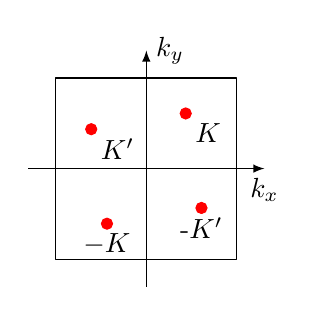
\begin{tikzpicture}[line join = round]
    \draw[] (-1.15,-1.15) rectangle (1.15,1.15);
    \draw[->] (-1.5,0) -- (1.5,0) node[anchor = north] {$k_x$};
    \draw[->] (0,-1.5) -- (0,1.5) node[anchor = west] {$k_y$};  
    \draw[fill, red] (0.5,0.7) node[black, anchor=north west] {$K$} circle (2pt) (-0.7,0.5) node[black, anchor=north west] {$K^\prime$} circle (2pt) (-0.5,-0.7) node[black, anchor=north] {$-K$} circle (2pt) (0.7,-0.5) node[black, anchor=north] {-$K^\prime$} circle (2pt);
\end{tikzpicture}
\end{document}